%%%%%%%%%%%%%%%%%%%%%%%%%%%%%%%%%%%%%%%%%
% Beamer Presentation
% LaTeX Template
% Version 1.0 (10/11/12)
%
% This template has been downloaded from:
% http://www.LaTeXTemplates.com
%
% License:
% CC BY-NC-SA 3.0 (http://creativecommons.org/licenses/by-nc-sa/3.0/)
%
%%%%%%%%%%%%%%%%%%%%%%%%%%%%%%%%%%%%%%%%%

%----------------------------------------------------------------------------------------
%	PACKAGES AND THEMES
%----------------------------------------------------------------------------------------

\documentclass{beamer}

\mode<presentation> {

    % The Beamer class comes with a number of default slide themes
    % which change the colors and layouts of slides. Below this is a list
    % of all the themes, uncomment each in turn to see what they look like.

    %\usetheme{default}
    %\usetheme{AnnArbor}
    %\usetheme{Antibes}
    %\usetheme{Bergen}
    %\usetheme{Berkeley}
    %\usetheme{Berlin}
    %\usetheme{Boadilla}
    %\usetheme{CambridgeUS}
    %\usetheme{Copenhagen}
    %\usetheme{Darmstadt}
    %\usetheme{Dresden}
    %\usetheme{Frankfurt}
    %\usetheme{Goettingen}
    %\usetheme{Hannover}
    %\usetheme{Ilmenau}
    %\usetheme{JuanLesPins}
    %\usetheme{Luebeck}
    \usetheme{Madrid}
    %\usetheme{Malmoe}
    %\usetheme{Marburg}
    %\usetheme{Montpellier}
    %\usetheme{PaloAlto}
    %\usetheme{Pittsburgh}
    %\usetheme{Rochester}
    %\usetheme{Singapore}
    %\usetheme{Szeged}
    %\usetheme{Warsaw}

    % As well as themes, the Beamer class has a number of color themes
    % for any slide theme. Uncomment each of these in turn to see how it
    % changes the colors of your current slide theme.

    %\usecolortheme{albatross}
    %\usecolortheme{beaver}
    %\usecolortheme{beetle}
    %\usecolortheme{crane}
    %\usecolortheme{dolphin}
    %\usecolortheme{dove}
    %\usecolortheme{fly}
    %\usecolortheme{lily}
    %\usecolortheme{orchid}
    %\usecolortheme{rose}
    %\usecolortheme{seagull}
    %\usecolortheme{seahorse}
    %\usecolortheme{whale}
    %\usecolortheme{wolverine}

    %\setbeamertemplate{footline} % To remove the footer line in all slides uncomment this line
    %\setbeamertemplate{footline}[page number] % To replace the footer line in all slides with a simple slide count uncomment this line

    %\setbeamertemplate{navigation symbols}{} % To remove the navigation symbols from the bottom of all slides uncomment this line
}

\usepackage[export]{adjustbox}
\usepackage{graphicx} % Allows including images
\usepackage{booktabs} % Allows the use of \toprule, \midrule and \bottomrule in tables
\graphicspath{ {./figures/} }


% Insert title slides
\AtBeginSection[]{
  \begin{frame}
  \vfill
  \centering
  \begin{beamercolorbox}[sep=8pt,center,shadow=true,rounded=true]{title}
    \usebeamerfont{title}\insertsectionhead\par%
  \end{beamercolorbox}
  \vfill
  \end{frame}
}

%----------------------------------------------------------------------------------------
%	TITLE PAGE
%----------------------------------------------------------------------------------------

\title[ESS-NW/CAR]{ESS-NW/CAR } % The short title appears at the bottom of every slide, the full title is only on the title page

\author{ Leon Fernandez, Jonas Ekman, Fredrik Hyyrynen, Jacob Kimblad, Yini Gao and  Yifan Ruan} % Your name
\institute[KTH] % Your institution as it will appear on the bottom of every slide, may be shorthand to save space
{
    MF2063 \\ % Your institution for the title page
    \medskip

}
\date{December 10, 2018} % Date, can be changed to a custom date

\begin{document}

\begin{frame}
    \titlepage % Print the title page as the first slide
\end{frame}

\begin{frame}
    \frametitle{Overview} % Table of contents slide, comment this block out to remove it
    \tableofcontents % Throughout your presentation, if you choose to use \section{} and \subsection{} commands, these will automatically be printed on this slide as an overview of your presentation
\end{frame}

%----------------------------------------------------------------------------------------
%	PRESENTATION SLIDES
%----------------------------------------------------------------------------------------

\section{Introduction and background} 
\begin{frame}
    \begin{figure}
        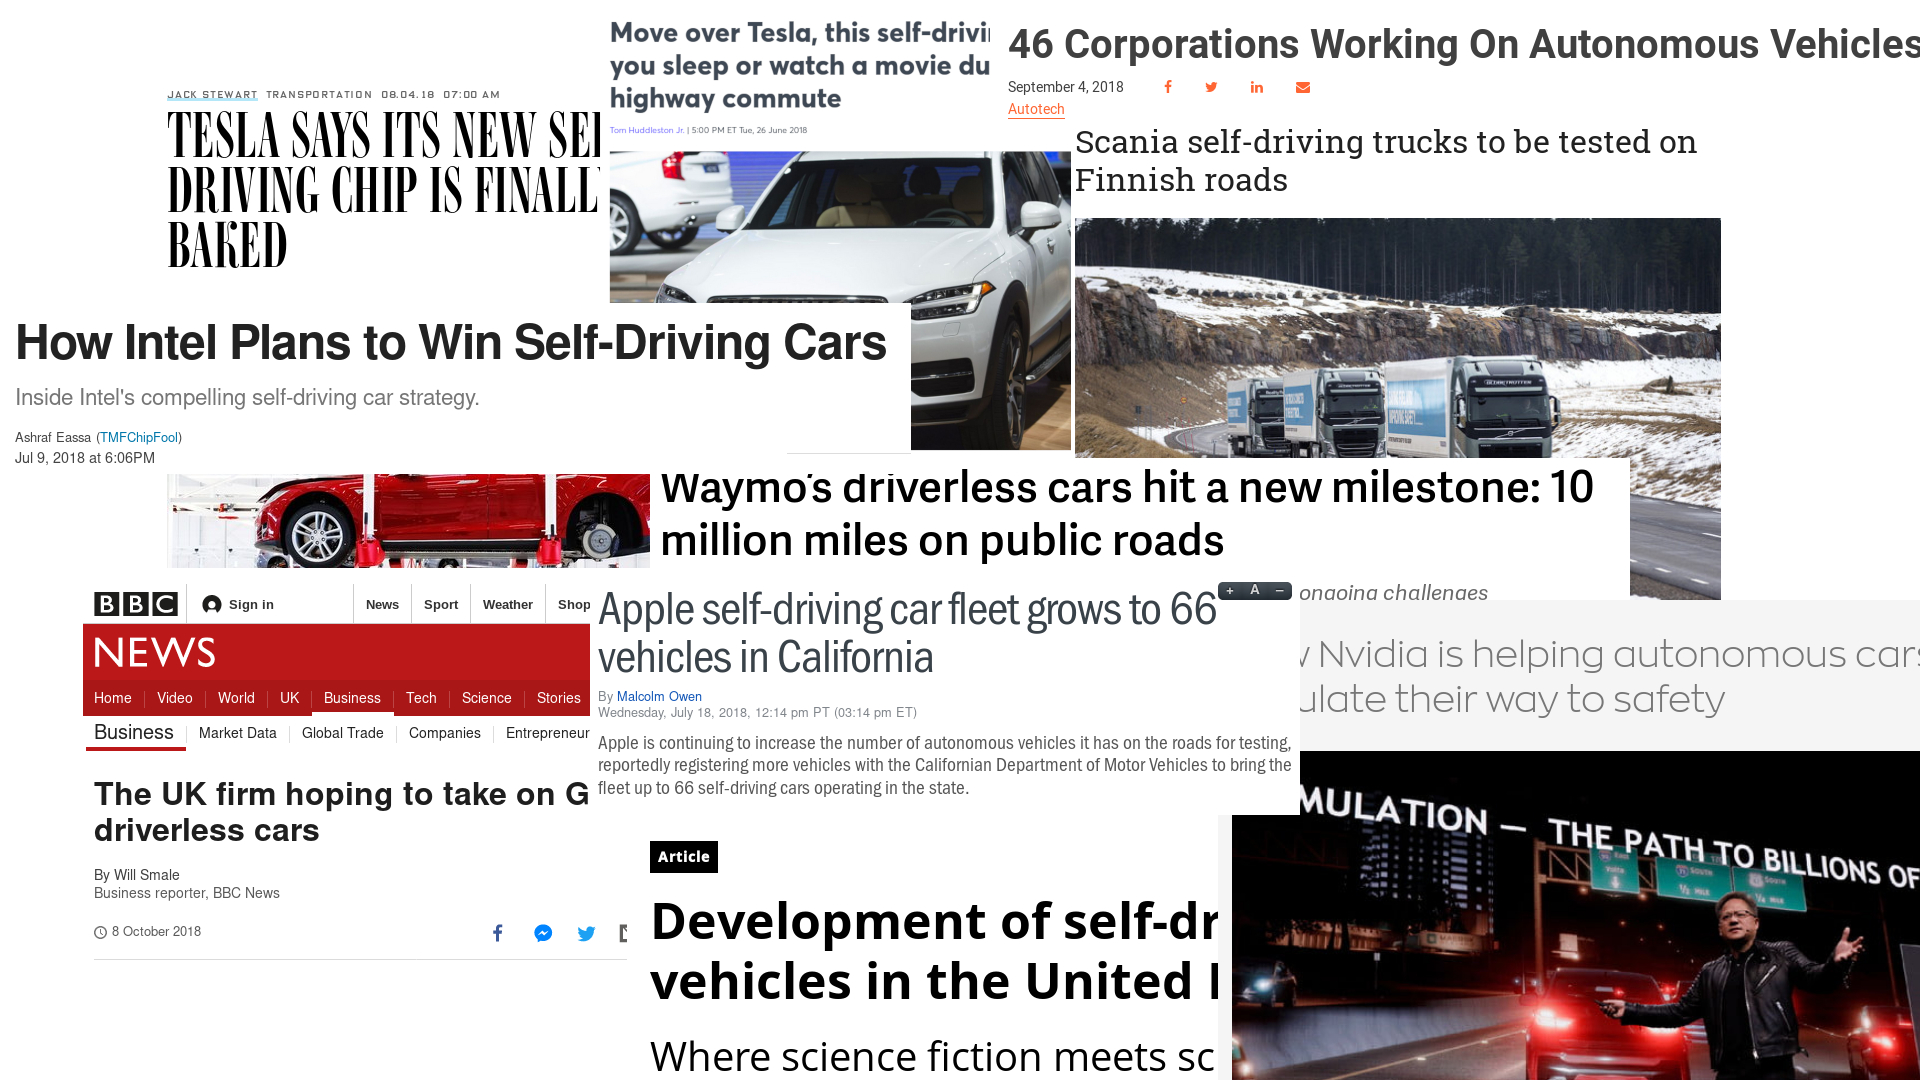
\includegraphics[width=1.2\linewidth]{articles.jpg}
    \end{figure}
\end{frame}

%------------------------------------------------
\subsection{Autonomous Driving}
\begin{frame}{Autonomous vehicles}
    \begin{itemize}
        \item Autonomous Driving (AD) and Advandced Driving Assistance Systems (ADAS)
        \item Common services:
            \begin{itemize}
                \item Object detection
                \item Speedometer
                \item Distance meter
                \item Cruise control
                \item Steering control
                \item Central decision making
            \end{itemize}
        \item Intelligent system monitoring:
            \begin{itemize}
                \item Startup
                \item Fault detection
                \item Communication surveilance
            \end{itemize}
        \item Dynamic adaptation:
            \begin{itemize}
                \item Failsafe behaviour
                \item Adaptive communication
            \end{itemize}
    \end{itemize}
\end{frame}


%------------------------------------------------

\subsection{Communication technologies}
\begin{frame}{The problem with existing communication technologies}
    \begin{itemize}
        \item Existing communication technologies between internal computers in cars:
            \begin{itemize}
                \item CAN (1 Megabit/s)
                \item LIN (19.2 Kilobit/s)
                \item FlexRay (10 Megabit/s)
            \end{itemize}

        \item Increased demand of bandwidth because of increased number of services in autnomous vehicles puts high demands on communication technologies.
        \item An interesting area of research is to use regular \textbf{ethernet }to replace existing communication technologies for cars.
            \begin{itemize}
                \item Current ethernet speeds reach into the Gigabit/s range.
            \end{itemize}
    \end{itemize}
    \begin{figure}
        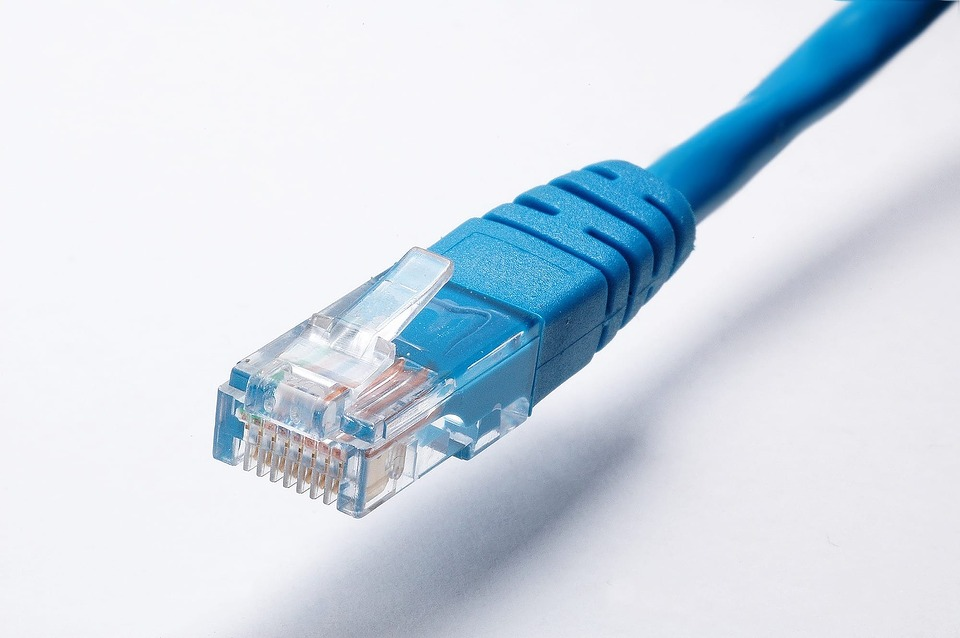
\includegraphics[width=0.3\linewidth]{ethernet_cable.jpg}
    \end{figure}
\end{frame}

%------------------------------------------------

\subsection{Ethernet}
\begin{frame}{The problem with ethernet}
    \begin{itemize}
        \item Ethernet is not developed for time-critical applications.
            \begin{itemize}
                \item Messages can take any road through the network.
                \item There is no way to give precedence for certain messages.
                \item Ethernet has no way to control for message congestion in the network.
                \item Worst-case latencies for messages can be to long because of congestion.
                    %Client server is slower than publish-subscribe
                \item Messaging is usually implemented using the client-server model.
                    %We cant do anything to change the control layer depending on existing circumstances
                \item Ethernet is unadaptive to real-time events.
            \end{itemize}
        \item An interesting area of research to tackle these problems is to use \textbf{Software Defined Networking }(SDN).
    \end{itemize}
\end{frame}

%------------------------------------------------

\subsection{Software defined networking}
\begin{frame}{Software defined networking}
    \begin{itemize}
        \item Builds onto the theory of regular ethernet.
        \item Move the intelligence from the switches to a central controller.
        \item The controller gather information from the switches.
        \item The controller decides how the traffic should be directed in the network.
        \item The SDN-controller allows for more adaptation in the network based on real-time events.
    \end{itemize}
    \begin{figure}
        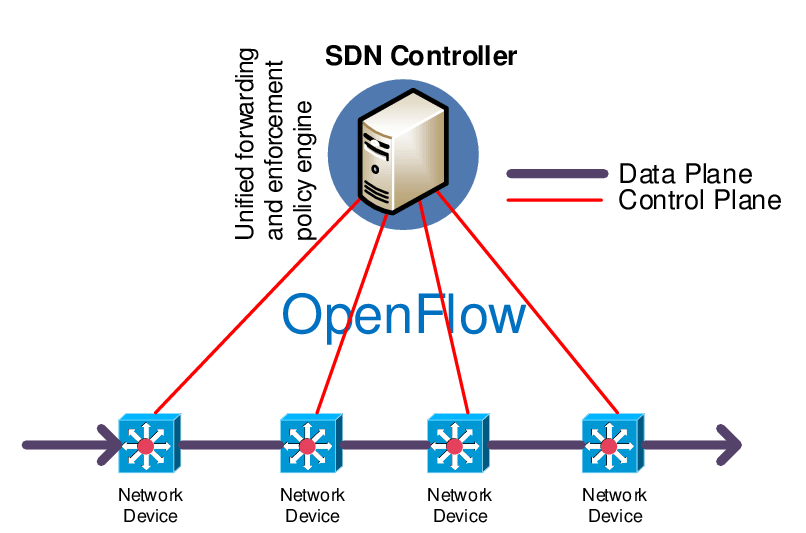
\includegraphics[width=0.55\linewidth]{sdn_info.png}
    \end{figure}
\end{frame}

%------------------------------------------------

\section{Our project}
\subsection{Goals}
\begin{frame}{Goals of the project}
    \begin{itemize}
        \item Produce a prototype of an SDN-based communication infrastructure for automotive vehicles.
        \item Produce a prototype of intelligent system monitoring and adaptation service for automotive vehicles.
        \begin{figure}
            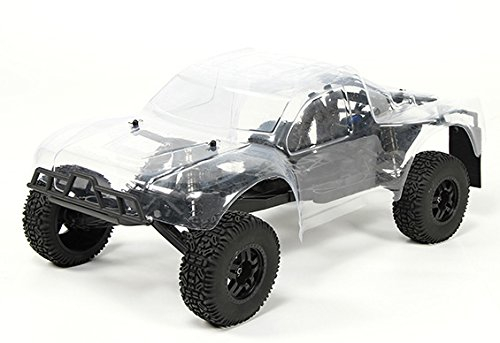
\includegraphics[width=0.5\linewidth]{turnigy_car.jpg}
            \caption{RC-car model kit used for the prototype}
        \end{figure}
    \end{itemize}
\end{frame}

%------------------------------------------------

\subsection{System architecture}
\begin{frame}{System architecture}
    \begin{figure}
        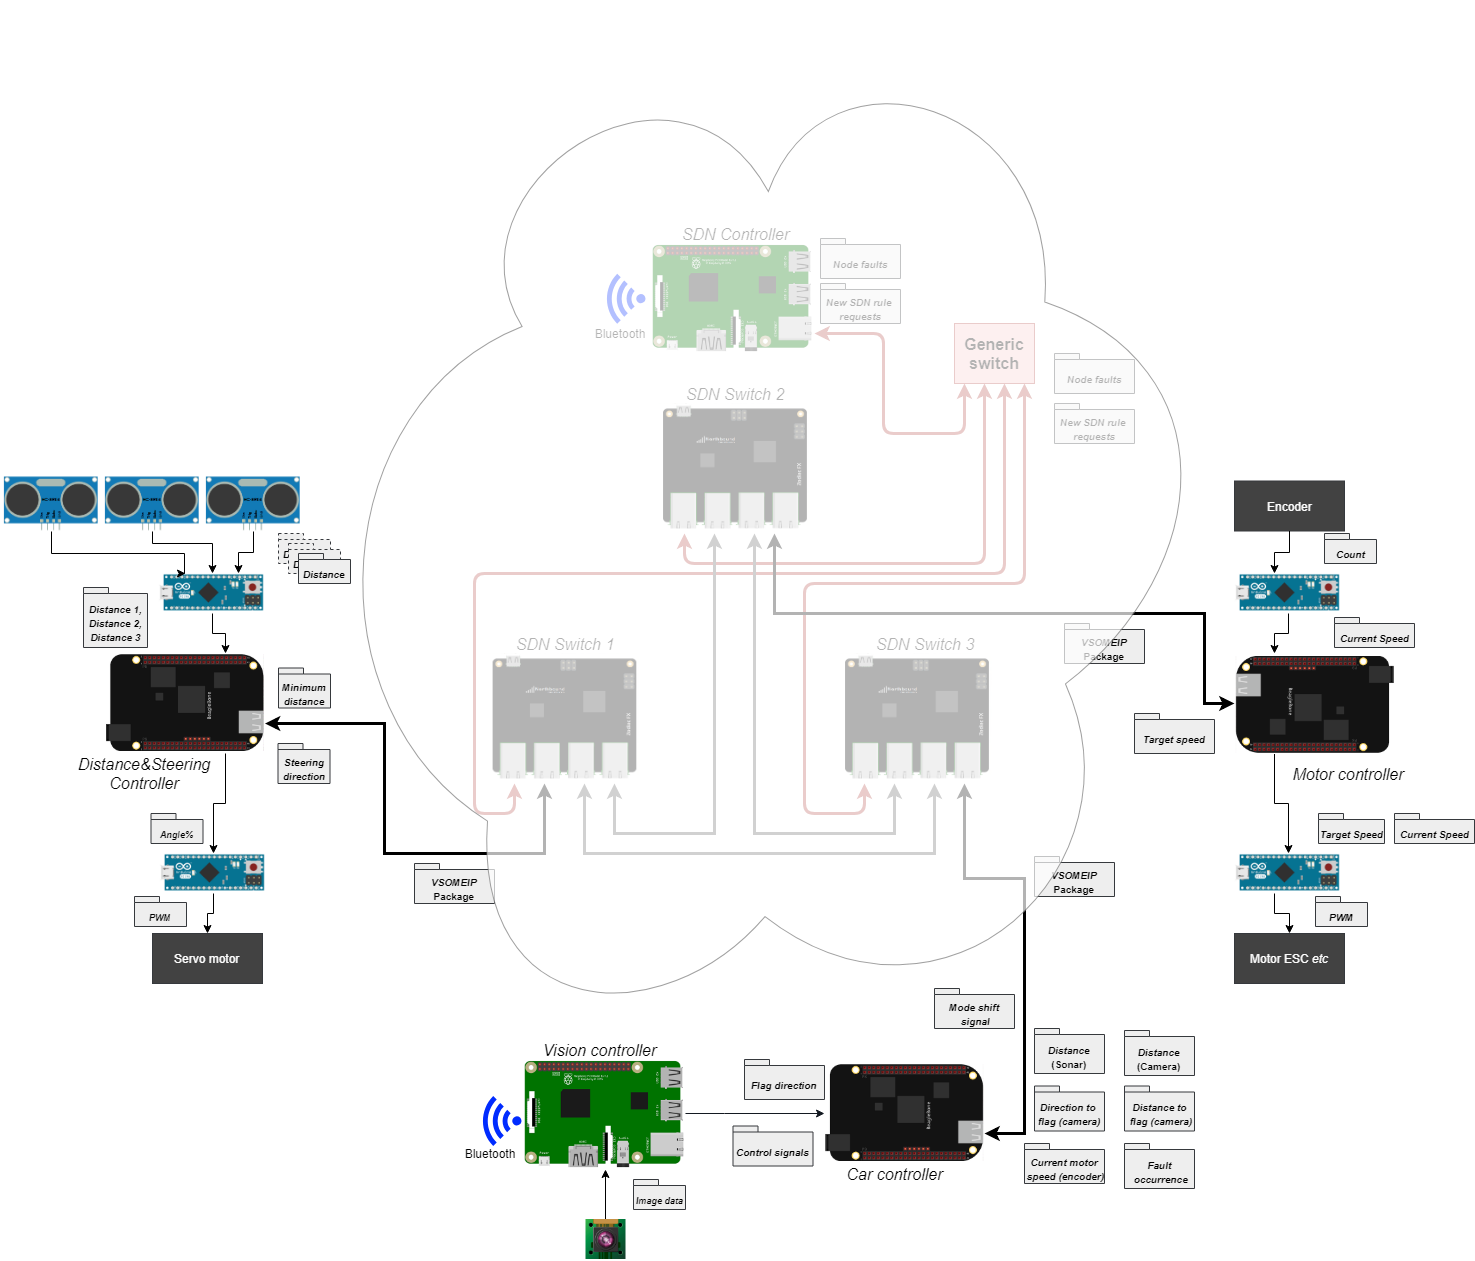
\includegraphics[width=0.75\linewidth]{network.png}
    \end{figure}
\end{frame}

%------------------------------------------------

\subsection{Implemented services}
\begin{frame}{Implemented services}
    \begin{itemize}
        \item Speedometer
        \item Cruise control
        \item Steering
        \item Object recognition
        \item 
    \end{itemize}
\end{frame}

\subsection{Hardware platform}

%------------------------------------------------

\section{Conclusion}
\begin{frame}{Conclusion}
    \begin{itemize}
        \item Ethernet is a promising candidate for increasing demand on bandwidth for communication in autonomous cars
        \item Ethernet is not without problems, many of which a SDN can help to solve.
        \item SDN networks allow for safe communications on autonomous vehicles by being fast, adaptive and customisable
        \item Fault detection and failsafe behaviour is a \textbf{must} in autonomous vehicles.
    \end{itemize}

\end{frame}

%------------------------------------------------

\section{old-slides}
\subsection{VSome/IP}
\begin{frame}{VSOME/IP}
    \begin{figure}
        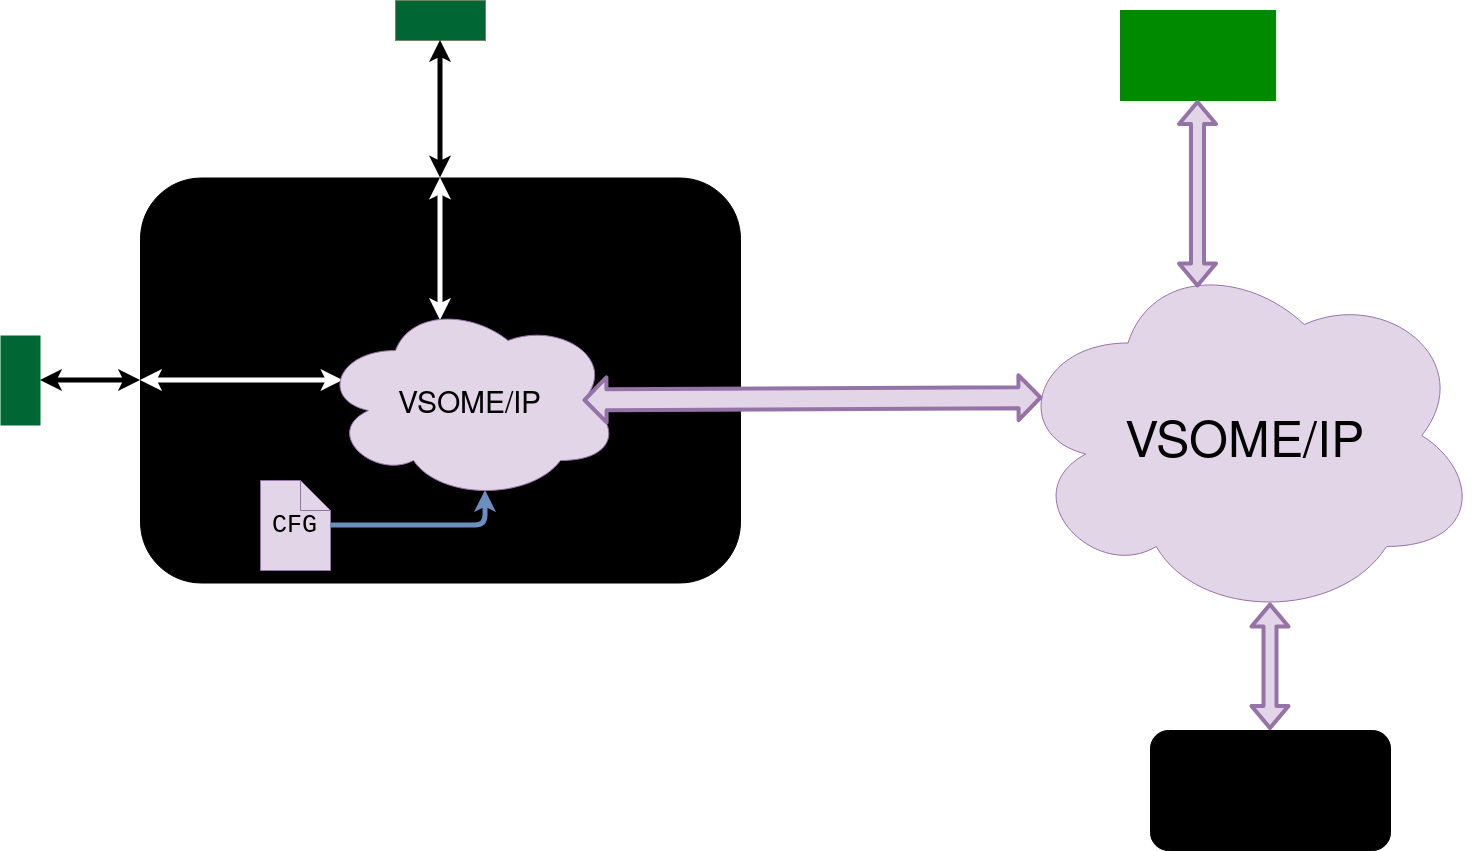
\includegraphics[width=\linewidth]{vsomeip.png}
    \end{figure}    
\end{frame}
%------------------------------------------------

\section{Control and sensors }
\subsection{Sensors}

\begin{frame}{Services}
    \begin{itemize}
        \item Ultrasonic sensor
            \begin{figure}
                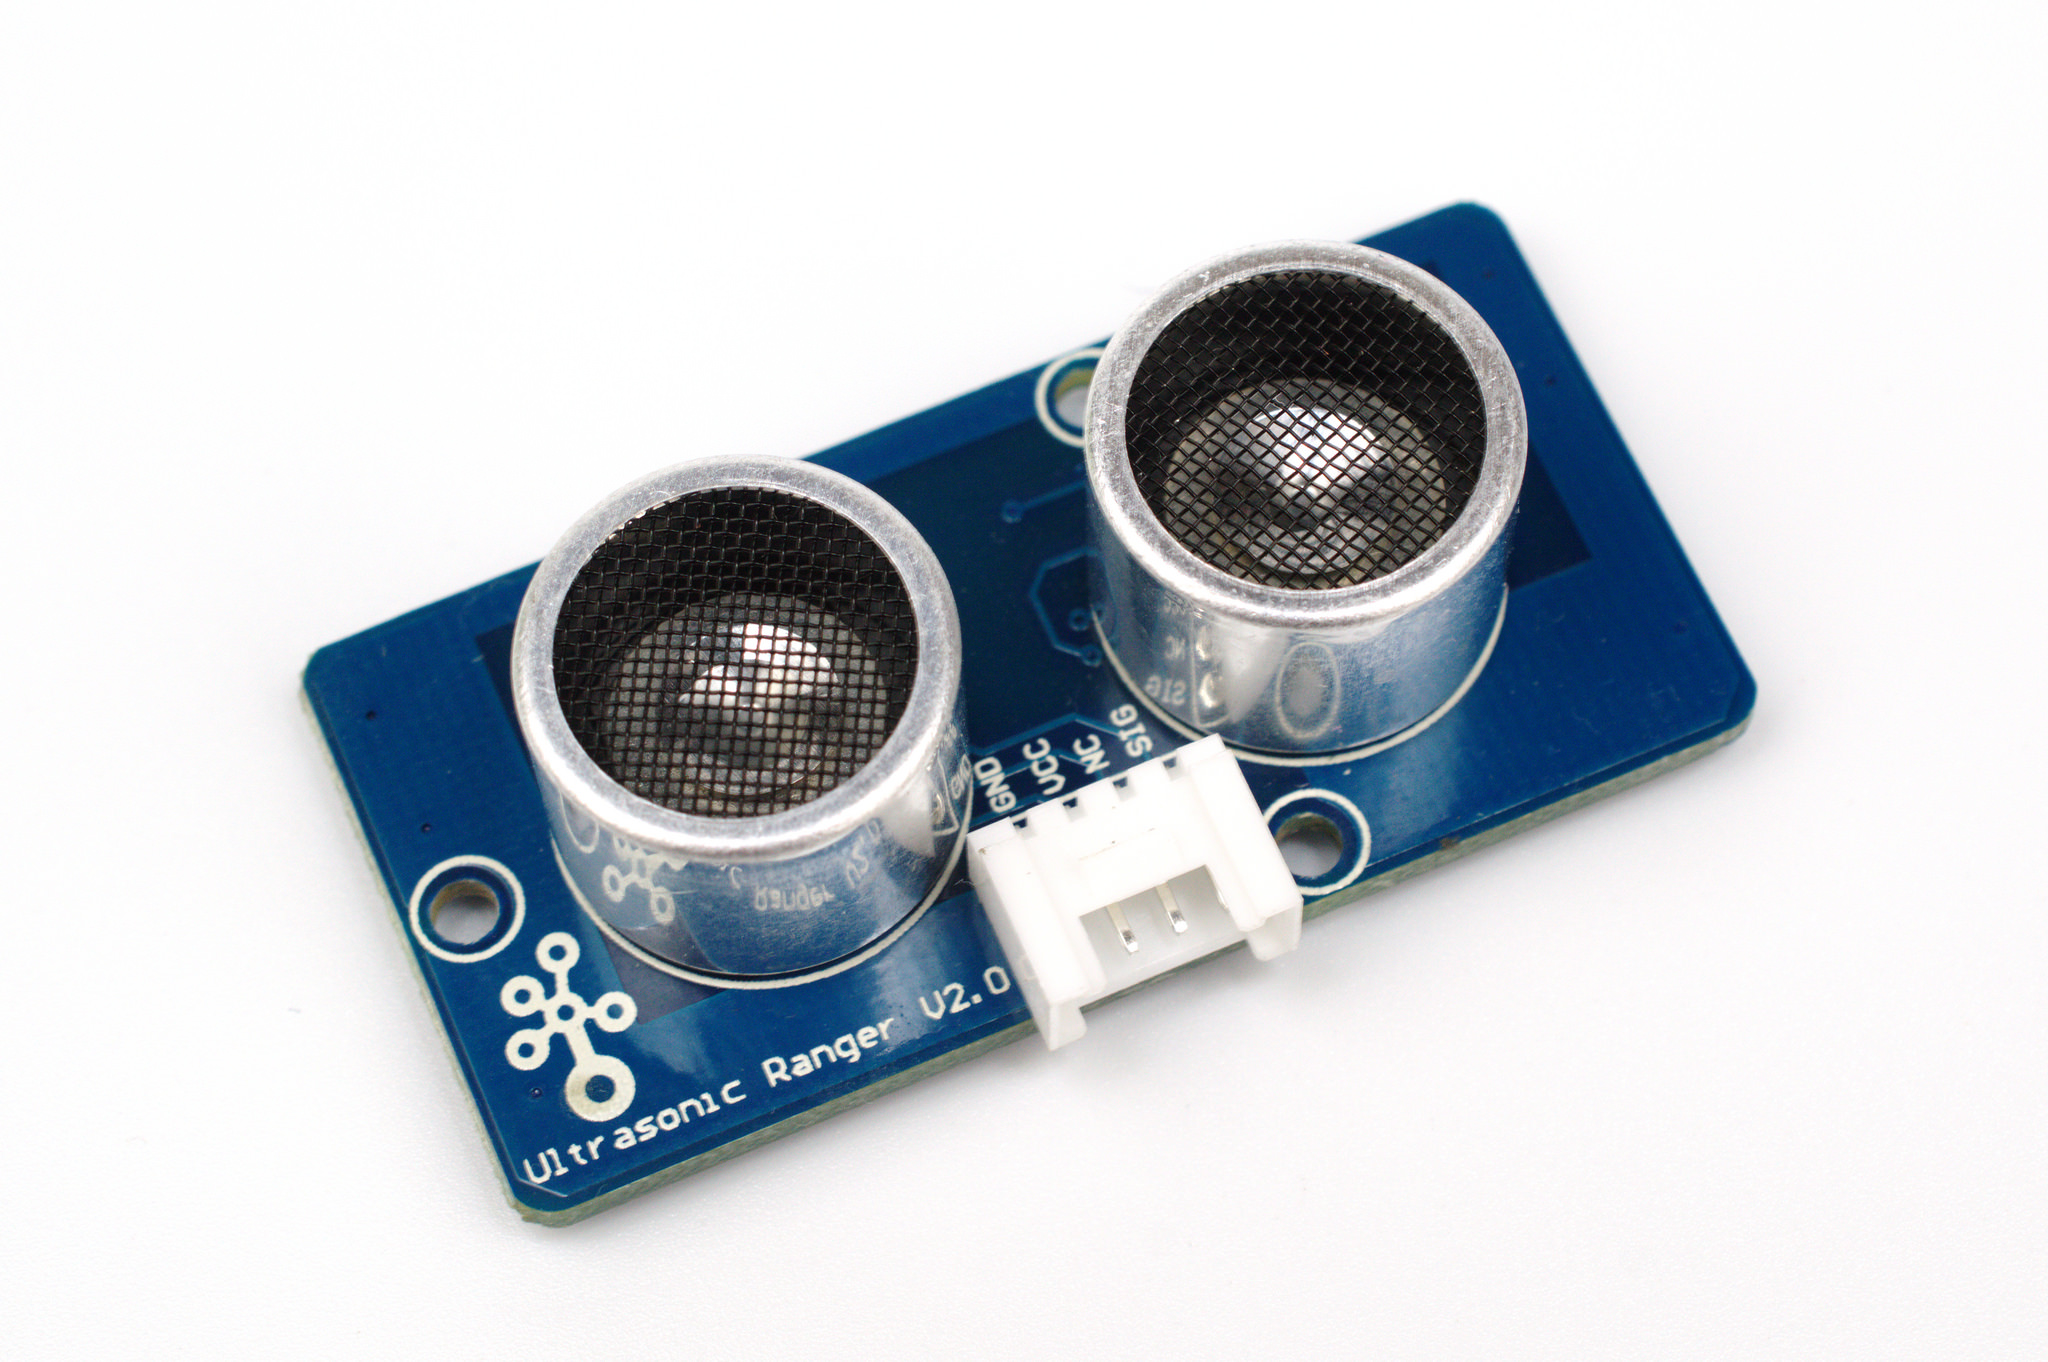
\includegraphics[width=0.2\linewidth, left]{ultrasonic.jpg}
            \end{figure}
        \item Reflective object sensor
            \begin{figure}
                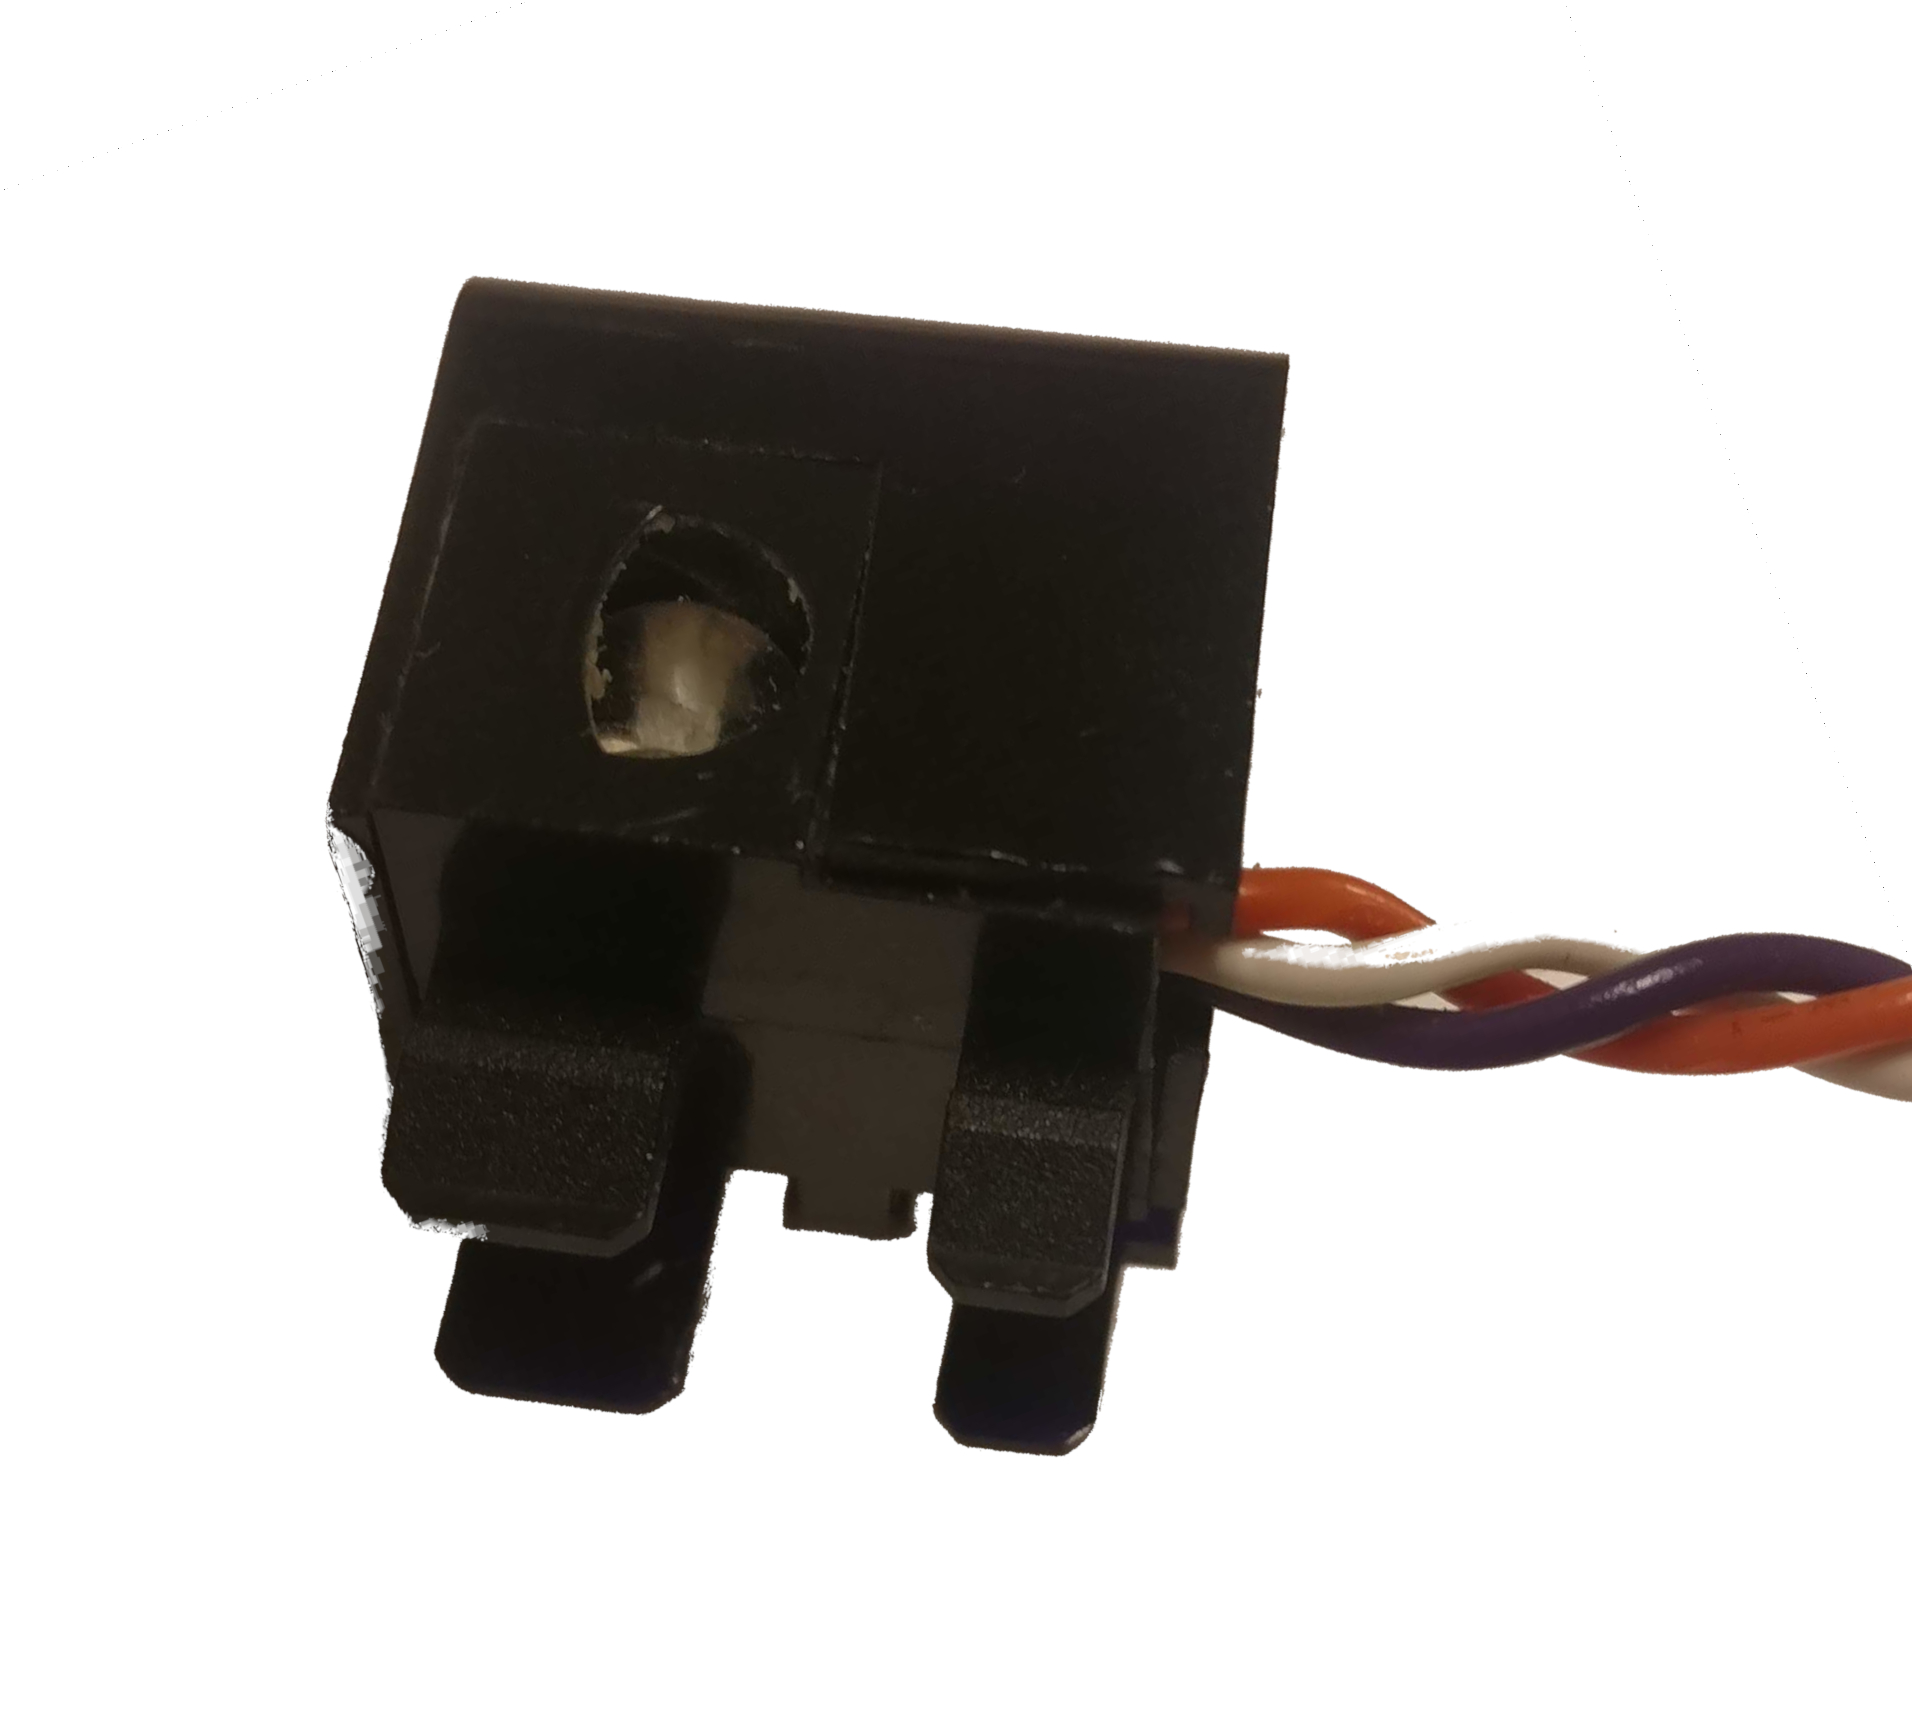
\includegraphics[width=0.2\linewidth, left]{ir.jpg}
            \end{figure}
        \item Camera
            \begin{figure}
                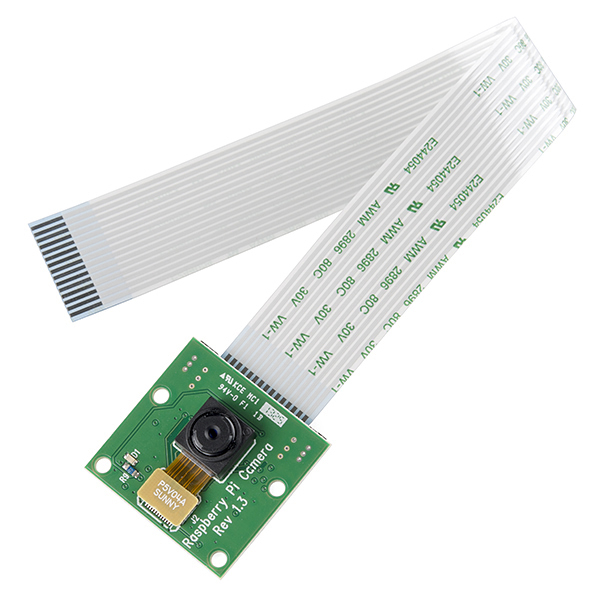
\includegraphics[width=0.2\linewidth, left]{camera.jpg}
            \end{figure}

    \end{itemize}

\end{frame}
%------------------------------------------------


\subsection{Actutators}
\begin{frame}{Actuators}
    \begin{itemize}
        \item Motor controller
        \item Steering controller
    \end{itemize}
    \begin{figure}
        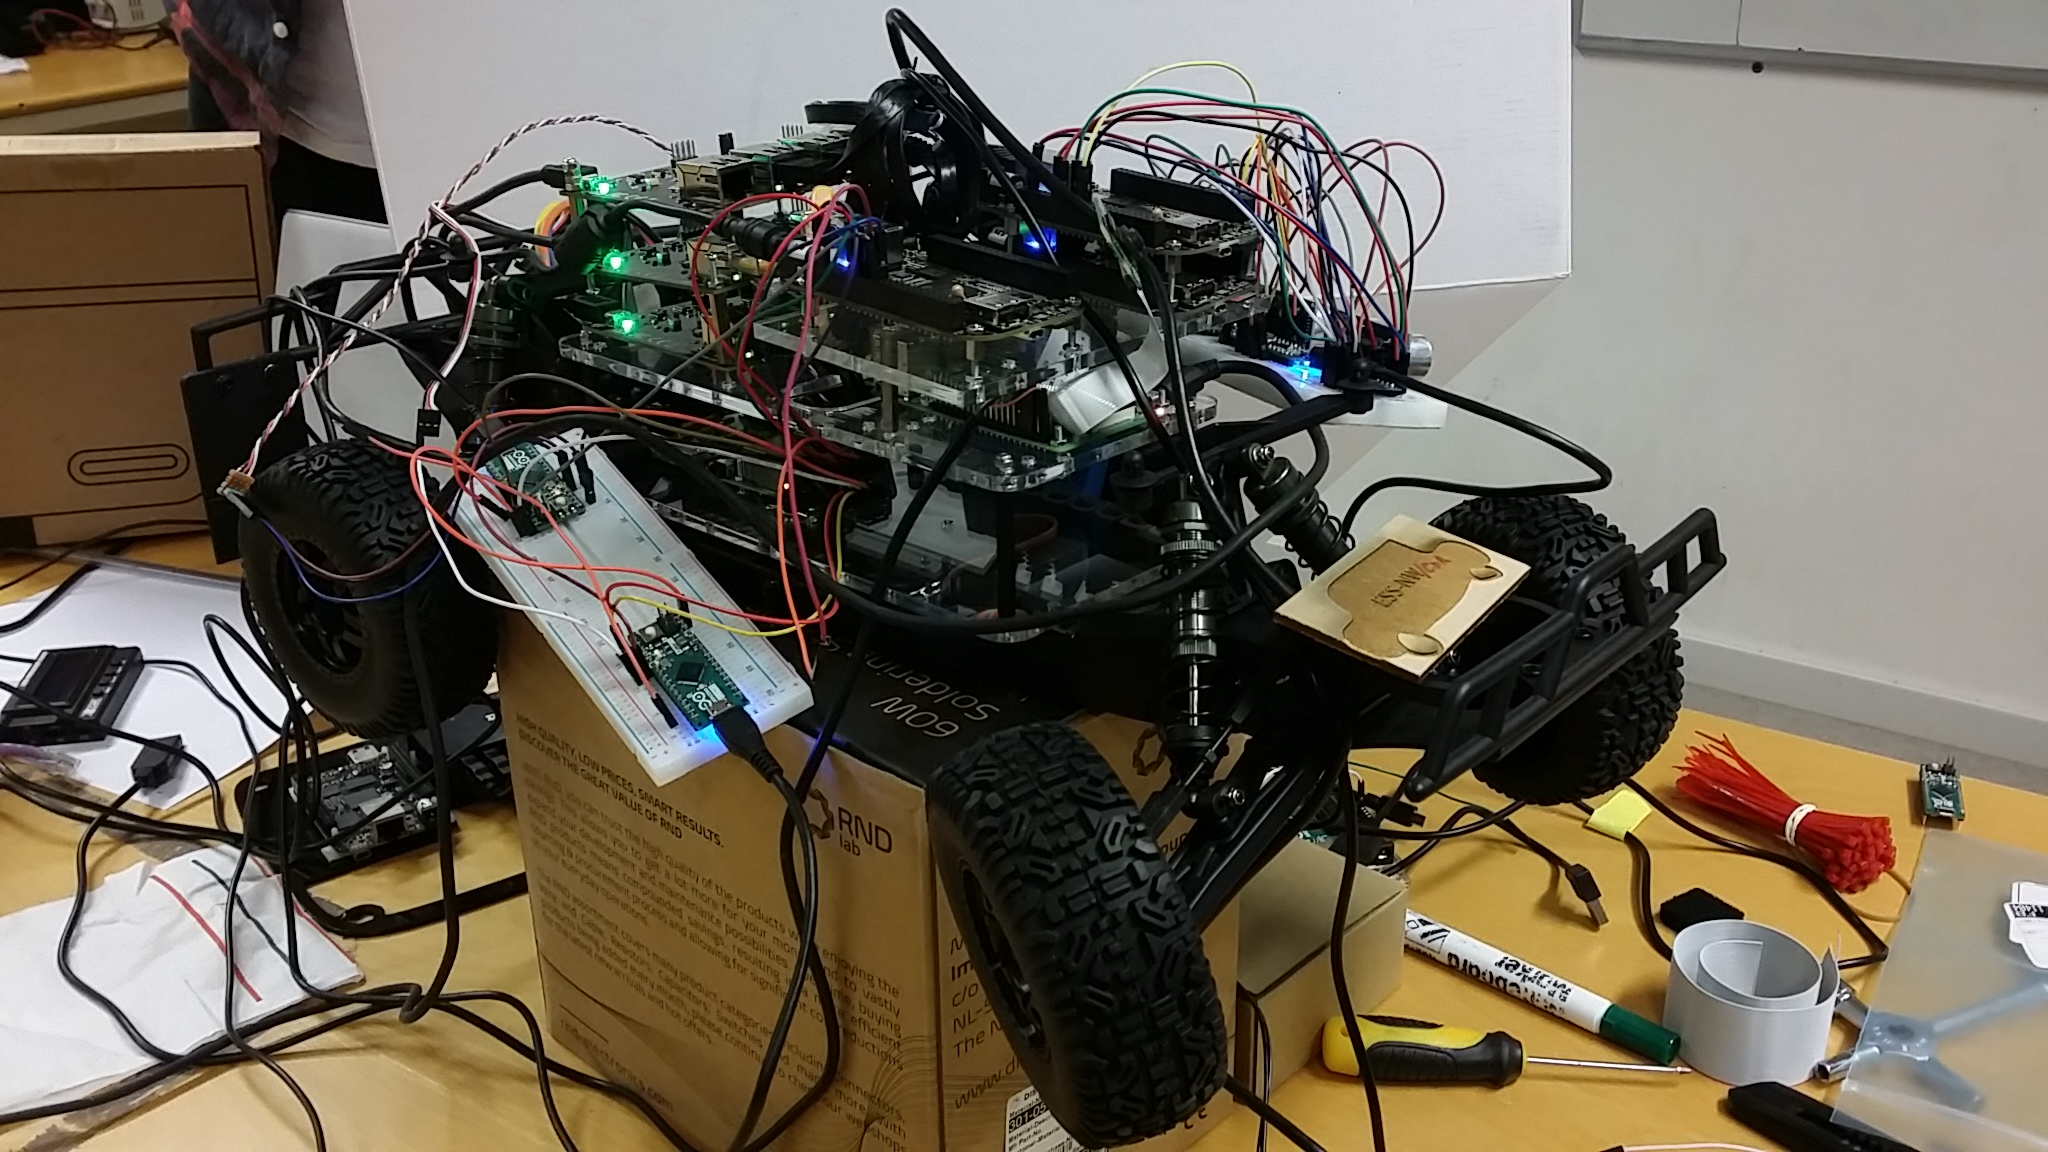
\includegraphics[width=0.6\linewidth, right]{car.jpg}
    \end{figure}
\end{frame}
%------------------------------------------------
\subsection{Autonomous behaviour}

\begin{frame}{Autonomous behaviour}
    \begin{itemize}
        \item Services
        \item State machine
            \begin{figure}
                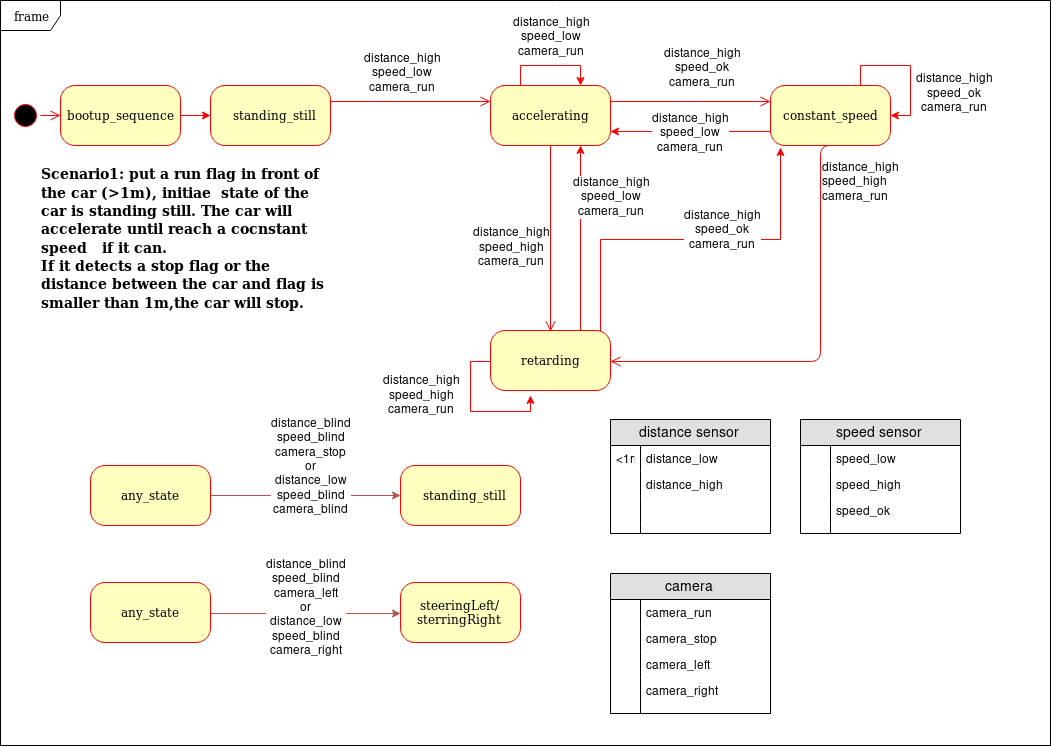
\includegraphics[width=0.7\linewidth]{statemachine.png}
                \caption{State machine}
            \end{figure}
    \end{itemize}

\end{frame}
%------------------------------------------------


\section{Assembly}
\subsection{Mounting}
\begin{frame}{The platform}

    \begin{columns}
        \begin{column}{0.47\textwidth}
            \begin{itemize}
                \item  Designed in Fusion 360
                \item  Cut out in the laser cutter
                \item  The idea of the design was to build up to get access to everything and to be modular
                \item Mounted on the car via two holes 
            \end{itemize}
        \end{column}
        \begin{column}{0.5\textwidth}
            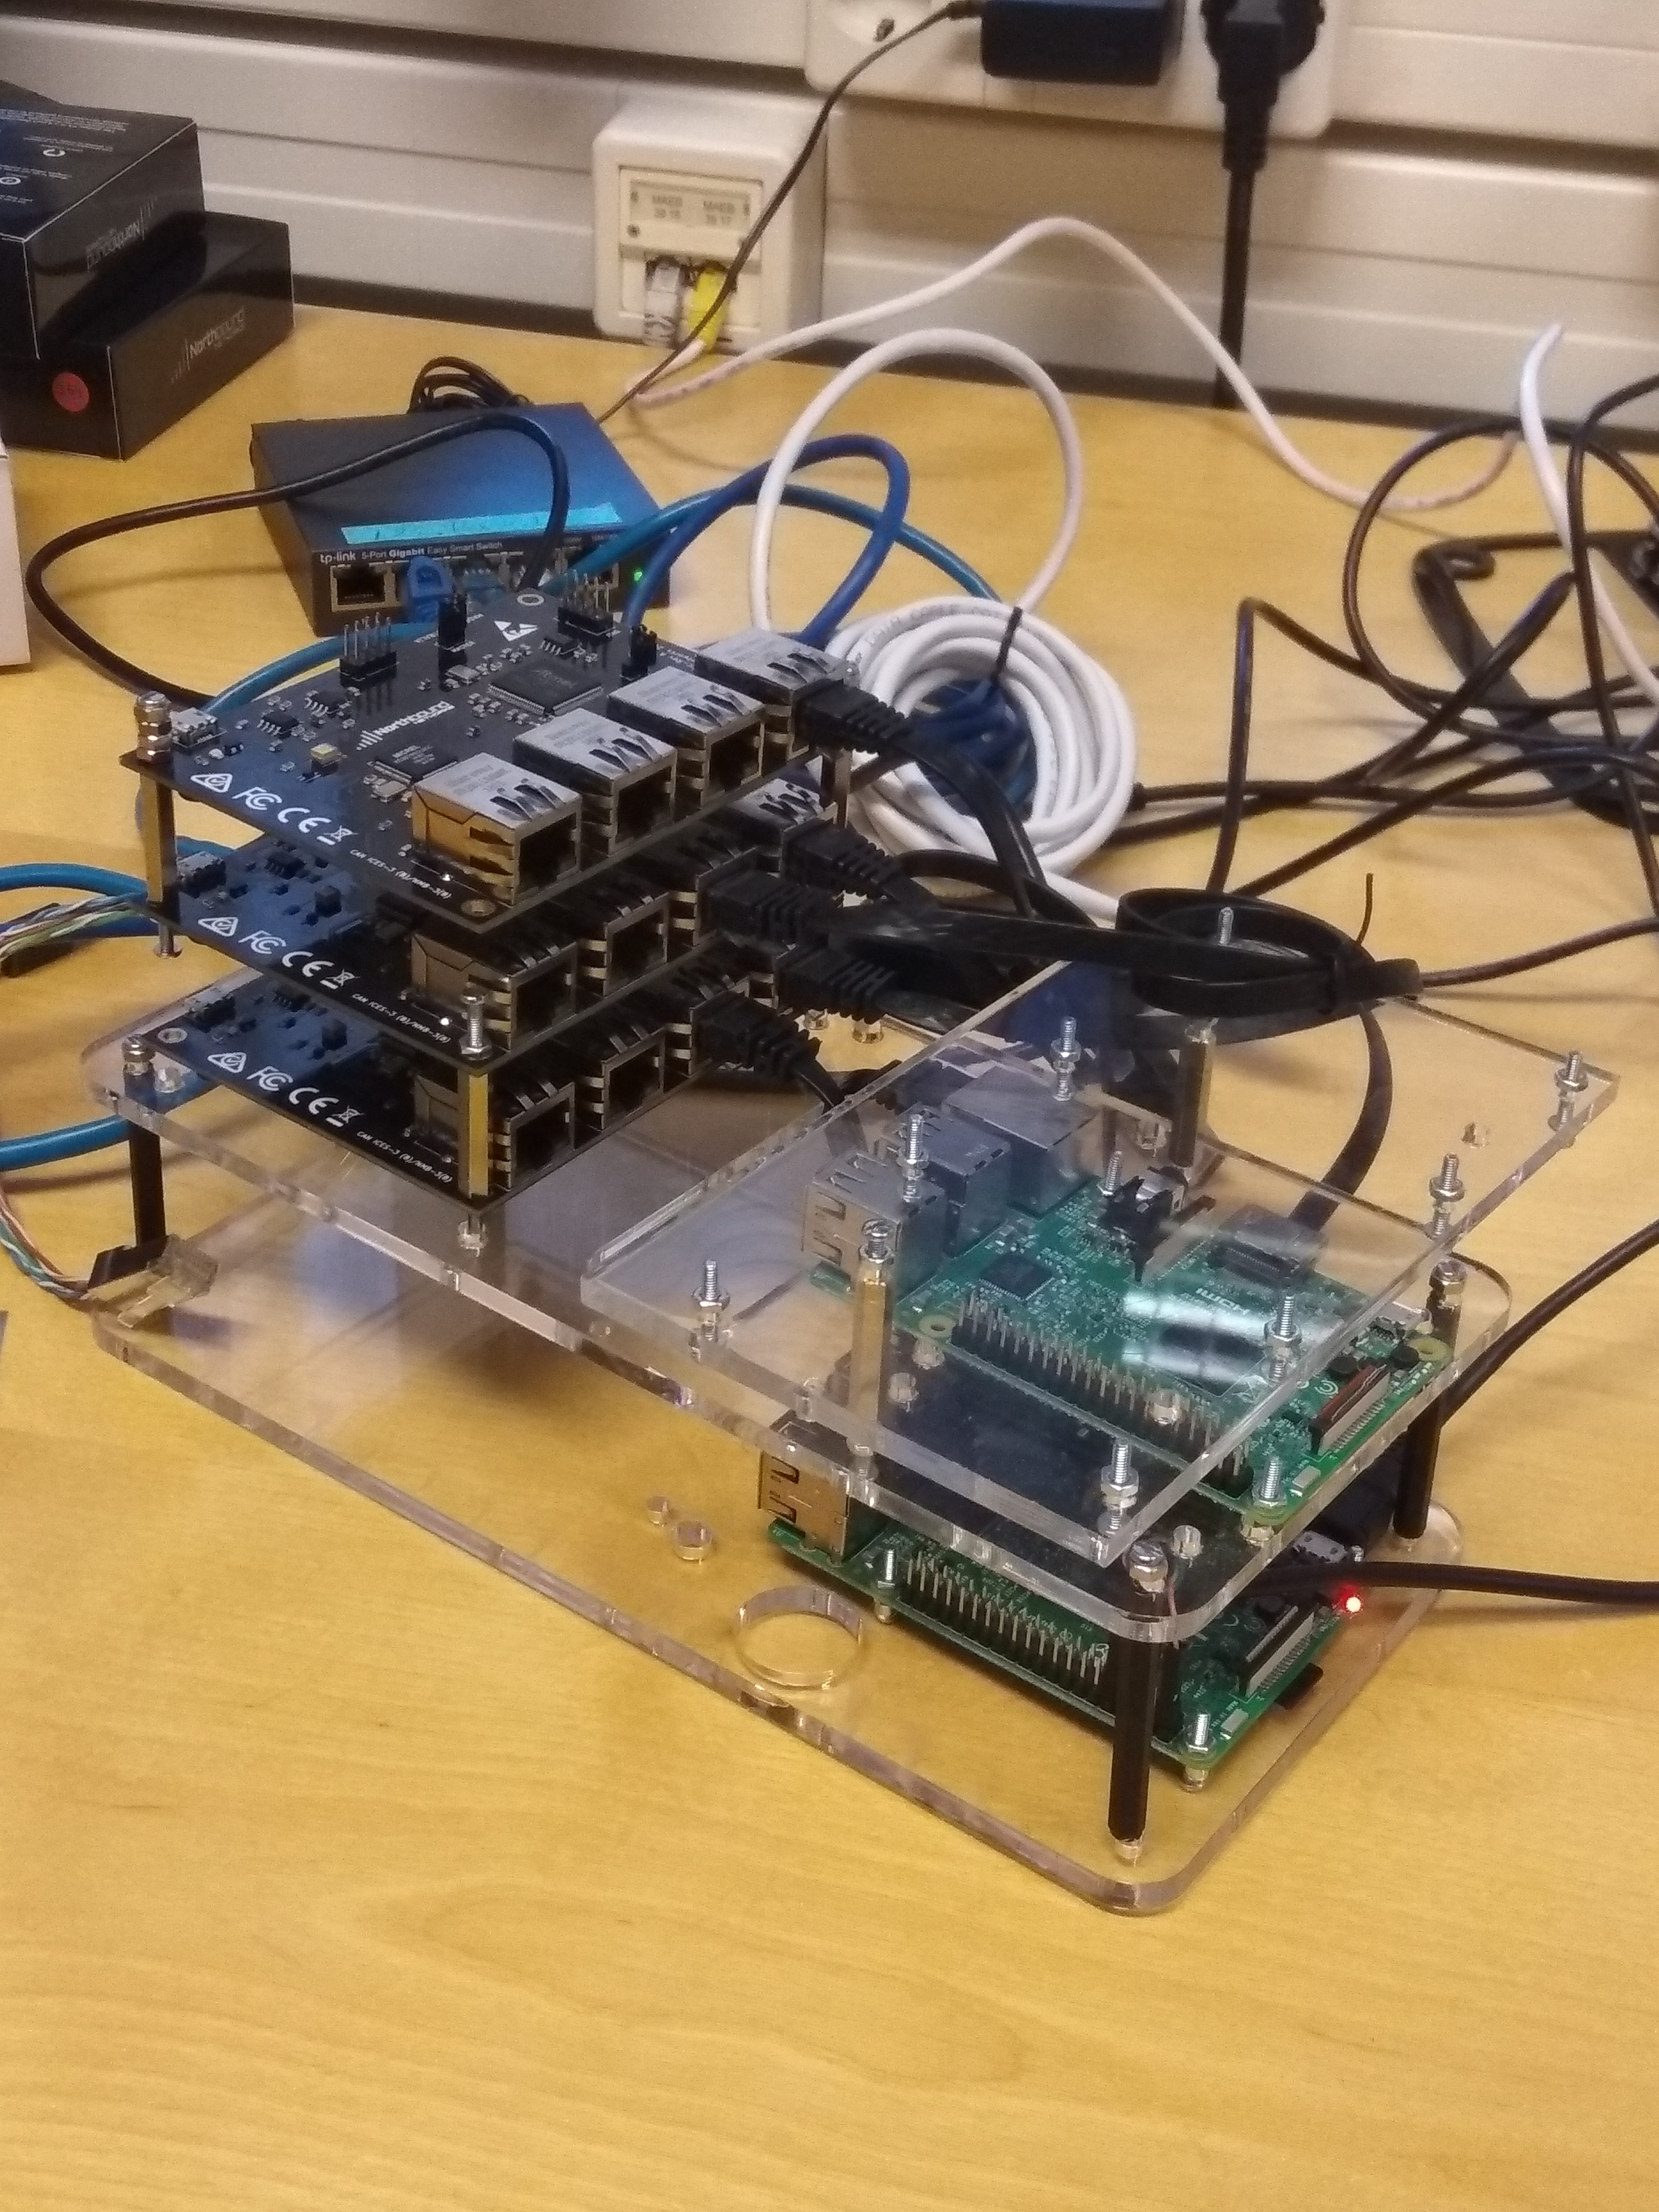
\includegraphics[width=0.7\linewidth]{platform.jpg}
            \label{fig:platform}
            %\caption{Platform}
        \end{column}
    \end{columns}
\end{frame}

%------------------------------------------------
\subsection{Power}
\begin{frame}{Power}
    \begin{itemize}
        \item We hade designed PCBs to mount the Arduinos on and to power the other devices
        \item Could not order PCB
        \item The machine PCB mill was broken both the one Mentorspace and proto Prototype Center
        \item Had to use breadboard 
    \end{itemize}
\end{frame}







%------------------------------------------------


%\begin{frame}
%\frametitle{References}
%\footnotesize{
%\begin{thebibliography}{99} % Beamer does not support BibTeX so %references must be inserted manually as below
%\bibitem[Smith, 2012]{p1} John Smith (2012)
%\newblock Title of the publication
%\newblock \emph{Journal Name} 12(3), 45 -- 678.
%\end{thebibliography}
%}
%\end{frame}

%------------------------------------------------

\begin{frame}
    \Huge{\centerline{Come check out our DEMO in the}} 
    \Huge{\centerline{prototyping lab on floor 3!}} 
\end{frame}

%----------------------------------------------------------------------------------------

        \end{document}
